We will now consider a complementary and equivalent approach to the path integral, based on the Fokker-Planck equation.
Rather than examining the trajectory point of view discussed by the Langevin-equation approach in the previous chapter,  we look at its ensemble statistics. Indeed, the Fokker-Planck equation describes the evolution of  $\mathcal{P}(x,t)$, the probability density to find a particle at position $x$ at time $t$. Similarly, one can define the conditional probability density $\mathcal{P}(x,t|x',t')$ of a particle being at $x$ at time $t$, given that it was at $x'$ at the earlier time $t'$. In the case where the particle is initialized at $x_0$ at time $t_0$, i.e., $\mathcal{P}(x,t_0)=\delta(x-x_0)$, it follows from Chapman-Kolmogorov equation that $\mathcal{P}(x,t)=\mathcal{P}(x,t|x_0,t_0)$.
In the following section, we derive the Fokker-Planck equation from the Kramers–Moyal expansion.

\section{Kramers-Moyal expansion}

%To derive the Kramers-Moyal expansion, consider a particle with a certain initial condition, so $\Pe(x, t = 0) = \delta(x)$.
%Then its probability distribution for later times \emph{equals} the conditional probability that it started at that point.
%That is, $\Pe(x, t) = \Pe(x, t| x = 0, t=0)$.
The derivation of the Fokker-Planck via the Kramers-Moyal expansion relies on the only assumptions that the underlying process is continuous and Markovian. Accordingly, we can start from the Chapman-Kolgomorov equation, \autoref{eq: chapman kolgomorov cont}, for a time-step $\Delta t$ is then
%
\begin{align}\label{eq: CK for KM}
    \Pe(x, t + \Delta t) = \int \dd x' \Pe(x, t + \Delta t|x',t) \Pe(x', t).
\end{align}
%
For later convenience, we now define the \emph{conditional moments},
%
\begin{align}
    K^{(n)}(x', t, \Delta t)
    =
    \E{\left[ x(t + \Delta t) - x(t) \right]^n}_{x(t) = x'}
    =
    \int \dd x \, (x - x')^n \Pe(x, t + \Delta t|x', t),
\end{align}
describing the moments of the amplitude of the typical displacement of the process in the time interval $\Delta t$ conditioned on the fact that it was at $x'$ at time $t$.
To derive the KM-expansion, we rewrite the delta-function as
%
\begin{align}
    \delta(y-x)
    = \delta(x' - x + y - x')
    & =
    \sum_{n = 0}^\infty
    \frac{1}{n!} (y - x')^n
    \left( \pdv{  }{ x' } \right)^n \delta(x' - x)\\
    & =
    \sum_{n = 0}^\infty
    \frac{(-1)^n}{n!} (y - x')^n
    \left( \pdv{  }{ x } \right)^n \delta(x' - x).
\end{align}
%
Here, we have Taylor-expanded the delta function, and change the variable with respect to which we differentiate in the last line.
The derivative of the Dirac-delta function is defined if we consider it in terms of an integral together with a test-function $f(x)$---we then integrate by parts, so
%
\begin{align}
    \int \dd x\, \delta'(x - x_0) f(x) = - \int \dd x\, \delta(x-x_0) f'(x) = - f'(x_0),
\end{align}
%
and so on.

Inserting the last expression into the trivial rewriting, 
%
\begin{align}
    \Pe(x, t + \Delta t| x', t) = \int \dd y\, \delta(y - x) \Pe(y, t + \Delta t | x', t).
\end{align}
%
we get
%
\begin{align}
    \Pe(x, t + \Delta t | x', t)
    & =
    \sum_{n = 0}^\infty
    \frac{(-1)^n}{n!} 
    \left( \pdv{  }{ x } \right)^n \delta(x' - x)
    \int \dd y \, (y - x')^n \Pe(y, t + \Delta t| x', t)\\
    & =
    \delta(x' - x) + 
    \sum_{n = 1}^\infty
    \frac{(-1)^n}{n!} 
    \left( \pdv{  }{ x } \right)^n \left[\delta(x' - x) K^{(n)}(x', t, \Delta t)\right].
\end{align}
%
Combining this rewriting with the Chapman-Kolgomorov, \autoref{eq: CK for KM}, and expanding in $\Delta t$, we get
%
\begin{align}
    \Pe(x, t + \Delta t) - \Pe(x, t) & = \Delta t \pdv{ \Pe(x, t) }{ t } + \Oh(\Delta t^2) \\
    & = \int \dd x' \Pe(x, t + \Delta t|x', t) \Pe(x', t) - \Pe(x, t) \\
    & = 
    \int \dd x' \,
    \left\{
        \delta(x' - x) + 
        \sum_{n = 1}^\infty
        \frac{(-1)^n}{n!} 
        \left( \pdv{  }{ x } \right)^n \left[\delta(x' - x) K^{(n)}(x, t, \Delta t)\right]
    \right\}
    \Pe(x', t)
    - \Pe(x, t)\\
    & = 
    \sum_{n = 1}^\infty
    \frac{(-1)^n}{n!} 
    \left( \pdv{  }{ x } \right)^n \left[\Pe(x, t) K^{(n)}(x, t, \Delta t)\right].
\end{align}
%
We define the \emph{Kramers-Moyal coefficients} as
%
\begin{align}
    \D^{(n)}(x, t) \equiv \lim_{\Delta t \rightarrow 0 } \frac{K^{(n)}(x, t, \Delta t)}{n! \Delta t},
\end{align}
%
which means that we can, in the limit $\Delta t\rightarrow 0$, write
%
\begin{align}
    \pdv{ \Pe(x, t) }{ t }
    =
    \sum_{n = 1}^\infty
    (-1)^n
    \left( \pdv{  }{ x } \right)^n \left[\Pe(x, t) \D^{(n)}(x, t)\right],
\end{align}
%
thus leading to the Kramers-Moyal equation.
Note that the coefficients $\mathcal{D}^{(n)}(x,t)$ are defined for $n$ integer larger then zero since $K^{(0)}=1$. They express the time variation of the $n$-th conditional moment of the amplitude of the infinitesimal step of the process. For simple Brownian motion, one expects $K^({1})=0$ (zero average displacement, similarly null for all odd-$n$ contributions), and $K^{(2)}\propto \Delta t$ (typical scaling of diffusion), while all other even moments $K^{(2n)}\propto (\Delta t)^n$ (show this with Wick theorem), implying that only $\mathcal{D}^{(2)}$ is non-null, thus retrieving the diffusion equation.
In general, it is possible to show that infinite KM expansion often features only a few non-vanishing contributions. This is rigorously expressed by \emph{Pawula's theorem}, which states that only three cases can occur for the Kramers-Moyal expansion:
\begin{itemize}
    \item[(1)] The series is truncated at $n = 1$, so $\D^{(n)} = 0$ for $n > 1$.
This corresponds to the deterministic evolution of $\Pe(x, t) = \delta(x - x(t))$, and the Kramers-Moyal equation becomes Liouville's equation.
\item[(2)] The series is truncated at $n = 2$. This gives the Fokker-Planck equation and will be what we concern ourselves with.

\item[(3)] The series is infinite, and any truncation leads to non-positive probability densities.
It is usually this in this case the equation is called the ``Kramers-Moyal equation''.
\end{itemize}



\begin{framed}
    \noindent
    \textit{Proof of Pawula's theorem:}
    We sketch the proof of the theorem here.
    It is based on (as in so many proofs) Schwartz inequality,
    %
    \begin{align}
        \left[
            \int \dd x\, p(x) f(x) g(x)
        \right]^2
        \leq
        \int \dd x\, p(x) f^2(x)
        \int \dd x\, p(x) g^2(x),
    \end{align}
    where $p(x)$ is a non-negative integrable function, and $g(x)$ and $f(x)$ are arbitrary integrable functions. You can think of $\int \mathrm{d}x p(x) f(x) g(x)$ as the scalar product of $f$ and $g$ defined on the (metric) functional space of integrable functions.
    %
    In this case, we choose $p(x) = \Pe(x', t, + \Delta t | x, t)$, and
    %
    \begin{align}
        f(x) & = 
        \begin{cases}
            (x - x')^{\frac{ m - 1 }{ 2 }}, & \text{if } m \text{ is odd and } m\geq 3\\
            (x - x')^{\frac{ m - 2 }{ 2 }}, & \text{if } m \text{ is even and } m\geq 4
        \end{cases},\\
        g(x) & = 
        \begin{cases}
            (x - x')^{\frac{ m + 1 }{ 2 }}, & \text{if } m \text{ is odd and } m\geq 3\\
            (x - x')^{\frac{ m + 2 }{ 2 }}, & \text{if } m \text{ is even and } m\geq 4
        \end{cases}.
    \end{align}
    %
    Then, the inequality becomes between conditional moments.
    On the left-hand side, switching $x'\rightarrow x$
    %
    \begin{align}
        \left[
            \int \dd x\, p(x) f(x) g(x)
        \right]^2
        = \left[K^m(x, t, \Delta t)\right]^2
    \end{align}
    %
    Consider $m$ even, then the right-hand side is
    %
    \begin{align}
        \int \dd x\, p(x) f^2(x)
        \int \dd x\, p(x) g^2(x)
        =
        K^{(m-1)}(x, t, \Delta t)
        K^{(m+1)}(x, t, \Delta t),
    \end{align}
    %
    so, applying with $ \lim_{\Delta t\rightarrow 0} \frac{ 1 }{ \Delta t^{2m} }$, the inequality becomes
    %
    \begin{align}
        \D^{(m)}(x, t) &\leq \frac{ (m-1)! (m+1)! }{ (m!)^2 } \D^{(m-1)}(x, t) \D^{(m+1)}(x, t),
        &&
        m \text{ odd and } m \geq 3.
    \end{align}
    %
    In the case of $m$ even, we instead get
    %
    \begin{align}
        \D^{(m)}(x, t) &\leq \frac{ (m-2)! (m+2)! }{ (m!)^2 } \D^{(m-2)}(x, t) \D^{(m+2)}(x, t),
        &&
        m \text{ even and } m \geq 4.
    \end{align}
    %
    We see now that the different coefficients are linked together in an infinite chain.
    We leave it as an exercise to show that if $\D^{(r)} = 0$ for any $r \geq 3$, then $\D^{(m)} = 0$ for all $m \geq 0$.
\end{framed}

\section{Connection to the Langevin equation}

As in the case of the simple Brownian motion discussed in the previous section, we would like to bridge the Langevin dynamics of continuous process to the corresponding Fokker-Planck equation.
For this purpose, it is convenient to consider the Langevin equation in the Itô discretization,
%
\begin{align}
    \odv{  }{ t } x(t)
    \overset{\alpha=0}{=}
    a_I(x(t), t) + b_I(x(t), t) \eta(t),
\end{align}
where $\eta(t)$ denotes the usual Gaussian white noise.
%
Then, it is easy to prove that the Kramers-Moyal coefficients are given by
%
\begin{align}
    D^{(1)}(x, t) & = a_I(x, t), &
    D^{(2)}(x, t) & = \frac{ 1 }{ 2 } b_I^2(x, t), &
    D^{(n)}(x, t) & = 0, \quad n > 2.
\end{align}
%
\begin{framed}
    \noindent
    \textit{Exercise:} Derive the Kramers-Moyal coefficients given above.
\end{framed}
We therefore get case (2) of Pawula's theorem, and the Kramers-Moyal equation reduces to the Fokker-Plank, which takes the form
%
\begin{align}
    \partial_t \Pe(x, t)
    = - \partial_x \left[a_I(x, t) \Pe(x, t)\right] + \frac{ 1 }{ 2 } \partial_x^2 \left[b_I(x, t)^2 \Pe(x, t)\right].
\end{align}
%
On the other hand, if we instead consider an equation with the Stratonovich discretization,
%
\begin{align}
    \odv{  }{ t } x(t)
    \overset{\alpha=\frac{1}{2}}{=}
    a_S(x(t), t) + b_S(x(t), t) \eta(t),
\end{align}
%
we have the following relationship, from the change-of-discrization formula \autoref{eq: change of discrtization},
%
\begin{align}
    a_I(x, t) &= a_S(x, t) + \frac{ 1 }{ 2 } b_S(x, t) \partial_x b_S(x, t), \\
    b_I(x, t) & = b_I(x, t).
\end{align}
%
Therefore, the corresponding Fokker-Planck is
%
\begin{align}
    \partial_t \Pe(x, t)
    & = - \partial_x \left[\left\{a_S(x, t) + \frac{ 1 }{ 2 } b_S(x, t) \partial_x b_S(x, t) \right\} \Pe(x, t)\right] 
    + \frac{ 1 }{ 2 } \partial_x^2 \left[b_S(x, t)^2 \Pe(x, t)\right] \\
    & = - \partial_x \left[a_S(x, t)  \Pe(x, t)\right] 
    + \frac{ 1 }{ 2 } \partial_x \left\{ b_S(x, t)\partial_x \left[ b_S(x, t) \Pe(x, t)\right] \right\}.
\end{align}
%
In higher dimensions, the Langevin equations, where $\bm x\in \R^n$ and $\bm \eta \in \R^m$,
%
\begin{align}
    \odv{  }{ t } x_i
    &\overset{\alpha=0}{=}
    - \partial_i a_{I,i}(\bm x, t) + B_{I,ij}(\bm x, t) \eta_j(t),\\
    \odv{  }{ t } x_i
    &\overset{\alpha=\frac{1}{2}}{=}
    - \partial_i a_{S,i}(\bm x, t) + B_{S,ij}(\bm x, t) \eta_j(t),\\
\end{align}
%
correspond to the following Fokker-Plancks:
%
\begin{align}
    \partial_t \Pe(\bm x, t) 
    & = - \partial_i \left[A_{I,i}(\bm x, t) \Pe(\bm x, t)\right]
    + \frac{ 1 }{ 2 } \partial_i \partial_j \left[B_{I, ik}(\bm x, t) B_{I, j k}(\bm x, t) \Pe(\bm x, t)\right], \\
    \partial_t \Pe(\bm x, t) 
    & = - \partial_i \left[A_{S,i}(\bm x, t) \Pe(\bm x, t)\right]
    + \frac{ 1 }{ 2 } \partial_i \left\{ B_{S, ik}(\bm x, t) \partial_j  \left[ B_{S, j k}(\bm x, t) \Pe(\bm x, t)\right] \right\},
\end{align}
%
where we have used Einstein's summation convention.


\subsection*{Underdamped equation}

If consider have an underdamped Langevin equation for a particle experiencing a force $-\bm \nabla U(\bm x)$,
%
\begin{align}
    \odv{  }{ t } \bm x(t) & = \bm v(t), \\
    m \odv{  }{ t } \bm v(t) &= - \gamma \bm v(t) - \bm \nabla U(\bm x(t)) + \sqrt{ 2 \gamma k_B T } \bm \eta(t),
\end{align}
%
where the noise is assumed to be uncorrelated for different components according to
%\begin{align}
$  \E{\eta_i(t) \eta_j(t')} = \delta_{ij} \delta(t-t')$,
%\end{align}
then the corresponding multi-dimensional Fokker-Planck equation is called \emph{Kramers equation}, and models the probability distribution of both velocity and position.

\subsection*{Overdamped equation}

In the limit $m/\gamma\rightarrow 0$, the above equation becomes an over-damped equation,
%
\begin{align}
    \odv{  }{ t } \bm x(t) &=  - \mu\bm \nabla U(\bm x(t)) + \sqrt{ 2 \mu k_B T } \bm \eta(t),
\end{align}
%
where $\mu = 1 / \gamma$ is the mobility.
The corresponding Fokker-Planck reads
%
\begin{align}
    \partial_t \Pe(\bm x, t)
    =
    \mu \bm \nabla \cdot \left[ \left(\bm \nabla U(\bm x) + k_B T \bm \nabla\right) \Pe(\bm x, t)\right].
\end{align}
%
Straight away, we get the Einstein relation $D = \mu k_B T$.
In case of equilibrium, the probability current $\bm J$, defined by $ \bm J= -\mu \left(\bm \nabla U(\bm x) + k_B T \bm \nabla\right) \Pe(\bm x, t) $, must vanish, thus yielding the Boltzmann distribution
%
%\begin{align}
    $\Pe(\bm x) = e^{- {U(\bm x)}/{k_B T} }$.
%\end{align}
%


\section{Wiener integral}

To connect this back to the path integral, we will now consider the \emph{Wiener} (or \emph{Brownian}) \emph{integral}.
If we consider a particle with Brownian motion initialized in the origin at $t = 0$, the probability distribution is, as we have seen earlier,
%
\begin{align}
    \Pe(x, t) = \Pe(x, t|0, 0)  = \frac{ 1 }{ \sqrt{ 4 \pi D t } } e^{-x^2/4 D t}.
\end{align}
%
%This is easily generalized, as
%
%\begin{align}
%    \Pe(x, t|x_0, t_0) = \Pe(x - x_0 , t - t_0|0, 0).
%\end{align}
%

\begin{figure}[!htb]
    \centering
    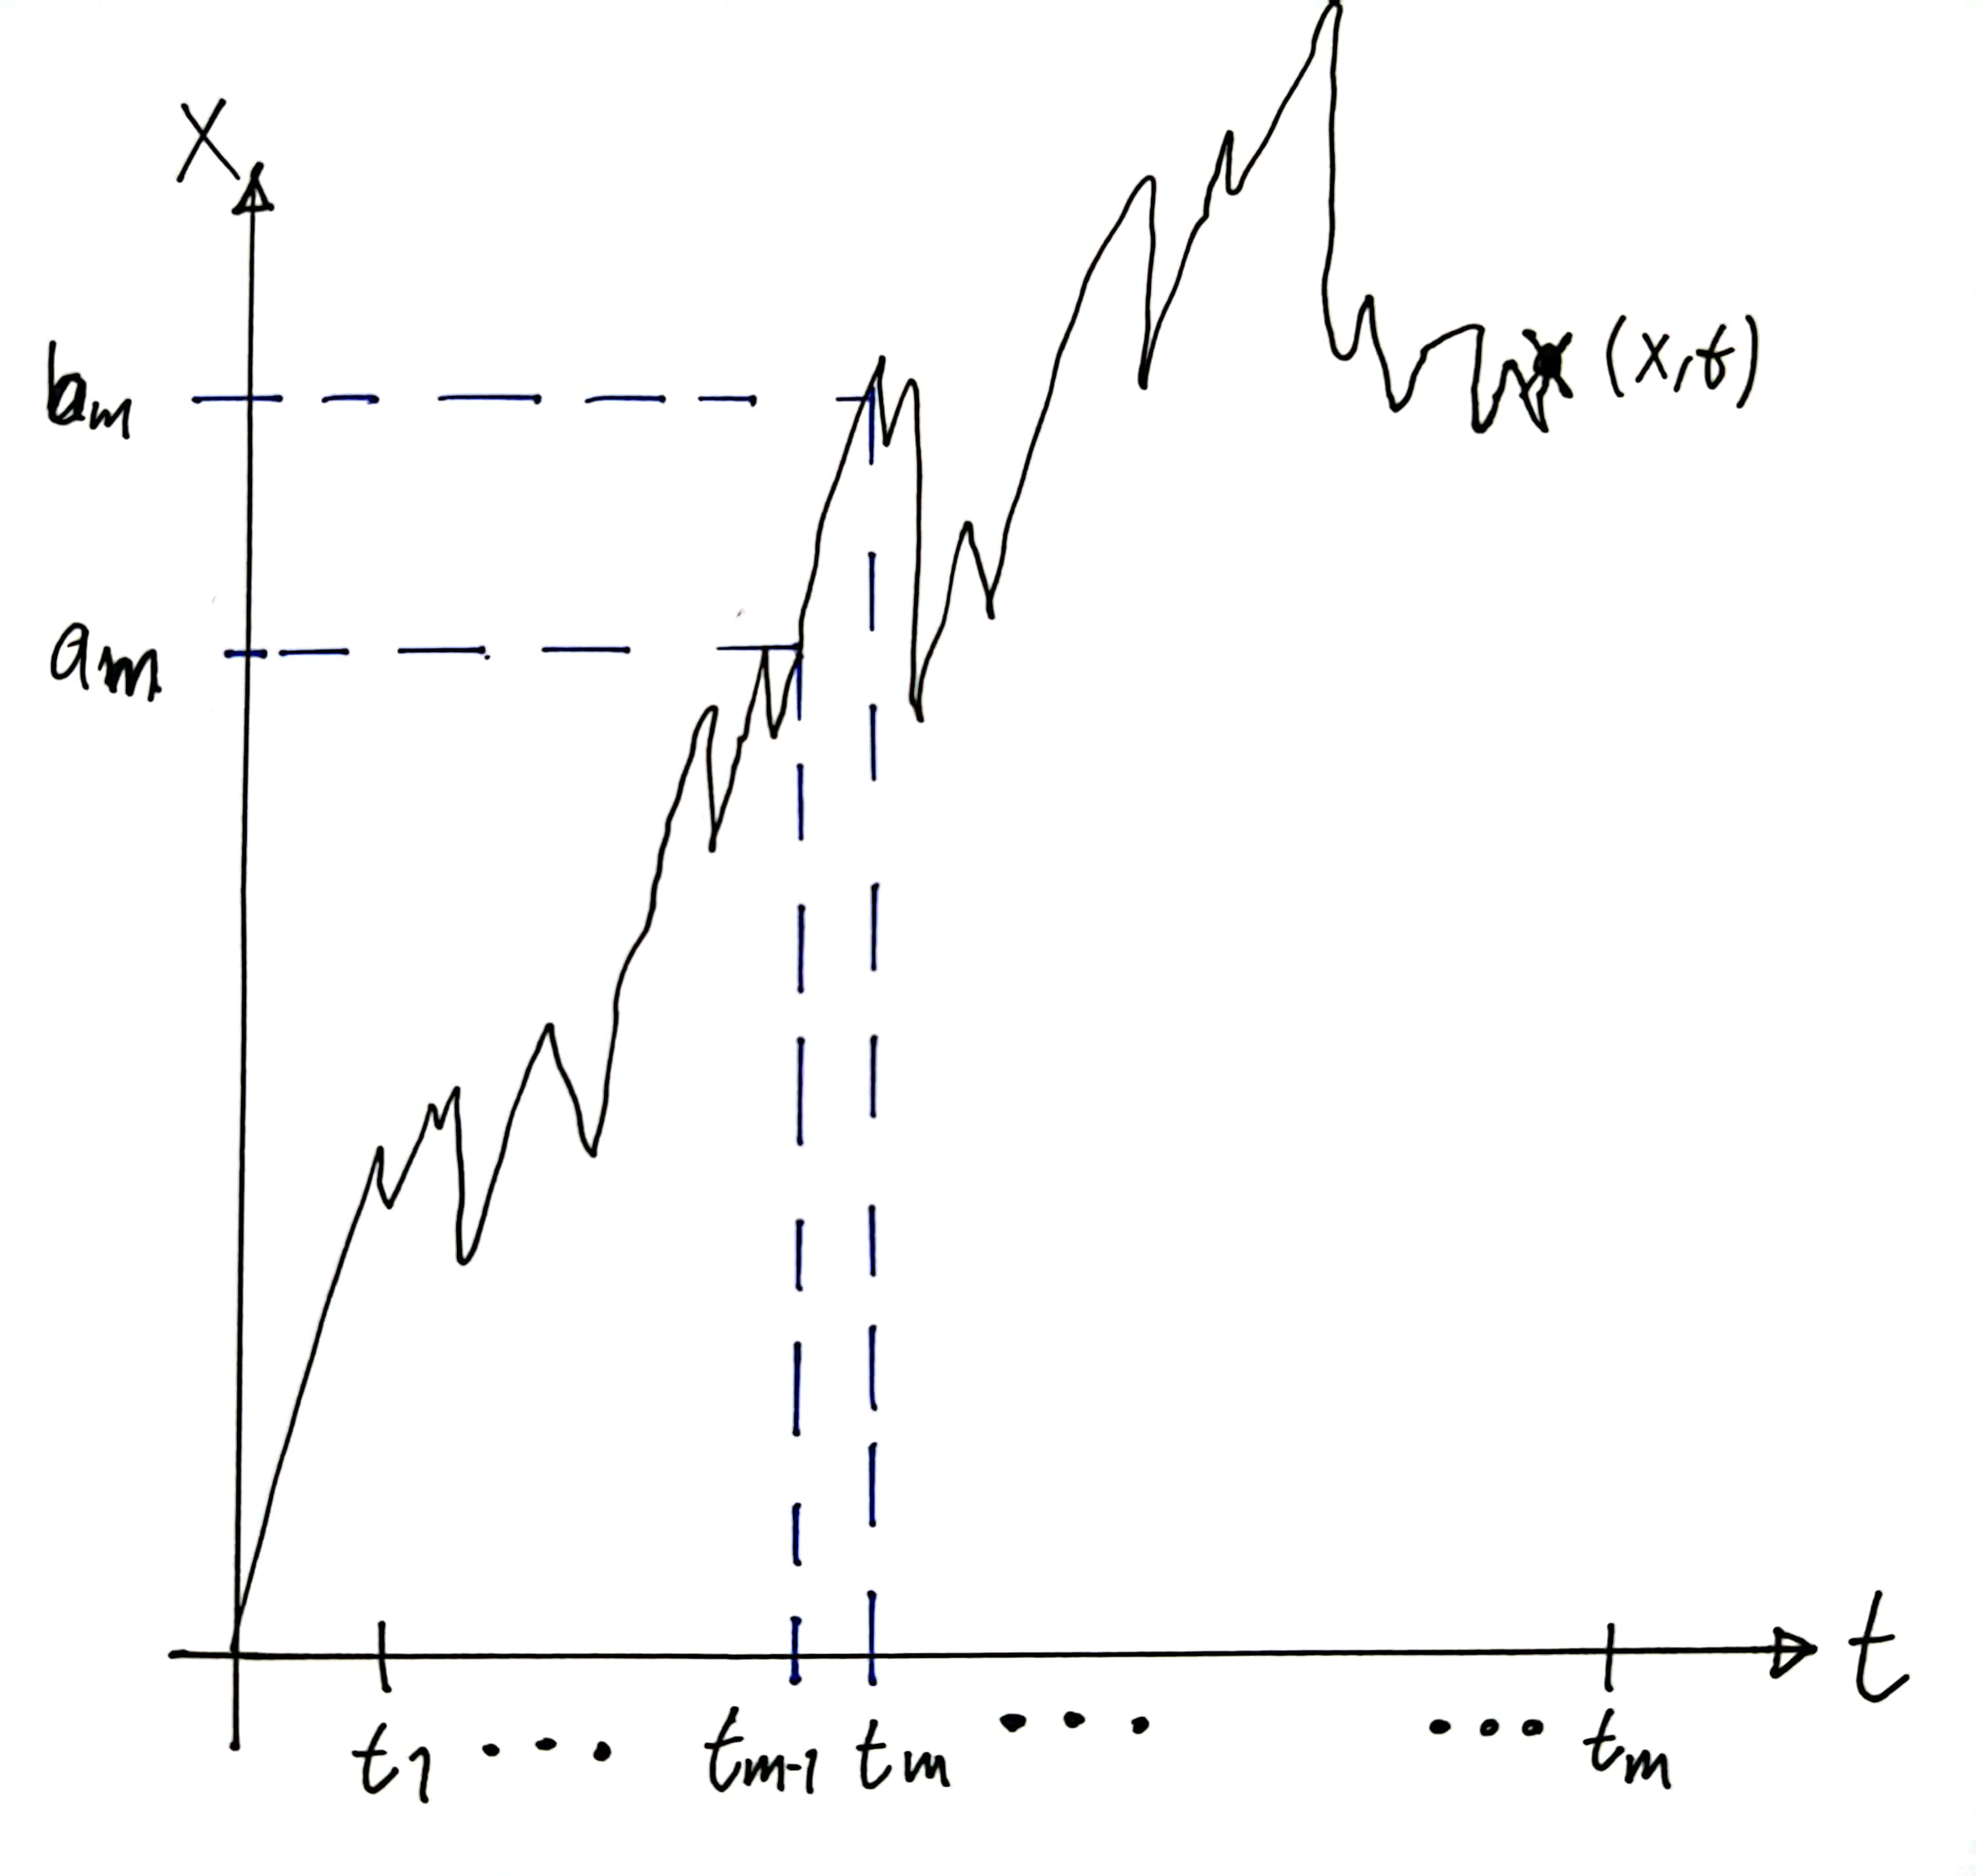
\includegraphics[width=.3\textwidth]{fig/path.jpg}
    \caption{A discretized path}
    \label{fig: path}
\end{figure}

As discussed around \autoref{eq: probability density}, when dealing with continuous space, and thus probability densities, the probability of finding a particle in the interval $(a, b)$ is
%
\begin{align}
    P(x\in (a, b), t ) = \int_a^b \dd x \, \Pe(\bm x, t).
\end{align}
%
To define probability density (``measure'') on an entire \emph{path}, and not just at isolated points, we discretize the path as
%
\begin{align}
    t_i &= i \Delta t, & i &\in [1, N], & t_N &= t, & x_i = x(t_i).
\end{align}
%
We consider paths with fixed endpoints, $x_0 = 0$, and $x_N = x$, as illustrated in \autoref{fig: path}.
A discretized path thus consists of finding the particle in certain intervals $(a_i, b_i)$ at times $t_i, i\in[1, N]$.
We define the probability measure of such a discretized path as
%
\begin{align}
    \Pe(x, t; x_i\in(a_i, b_i),\,  i \in 1, \cdots N )
    =
    \int\limits_{a_1}^{b_1} \dd x_1
    \cdots
    \int\limits_{a_{N-1}}^{b_{N-1}} \dd x_{N-1}\,
    \Pe(x, t | x_{N-1}, t_{N-1}) \cdots \Pe(x_{2}, t_{2} | x_{1}, t_{1}) \Pe(x_{1}, t_{1}) 
\end{align}
%
Then, in the continuum limit, this becomes Brownian integral,
%
\begin{align}
    \D x(t)
    \equiv
    \lim_{\substack{|a_i-b_i|\rightarrow 0\\N \rightarrow \infty \\ t = \const}}
    \Pe(x, t;  x_i\in(a_i, b_i),\,  i \in 1, \cdots N ).
\end{align}
%
This is a more careful definition of the path-integral measure defined in \autoref{section: introducing pi}.
In fact, this is a bonafide probability measure, as one can easily recognize the three fundamental ingredients characterizing a probability space:
%
\begin{enumerate}
    \item a \emph{sample space}: the space of all possible events, here given by the space of all continuous trajectories between two points at different times;
    \item a $\sigma$-algebra: all subsets of the sample space (endowed with a proper topological structure) that can be measured, here represented by the sets of all trajectories crossing all the intermediate $(a_i,b_i)$ sets;
    \item a measure on the sample space, which assigns a non-negative real number (probability) to every element of the $\sigma-$algebra, here given by the (normalized) Wiener integral.
\end{enumerate}
%

\subsection*{Brownian functional}

Suppose $Q[x]$ is some \emph{functional} of the paths $x(t)$ with the form
%
\begin{align}
    Q[x] = \exp \left\{ - \int_0^t \dd \tau \, U(x(\tau)) \right\}.
\end{align}
%
We have already encountered such a functional in the Onsager-Machlup functional.
This is called a \emph{Brownian functional}.
In discretized form, this is a function $Q(x_1, \cdots x_{N-1})$.
Then, the expectation of this functional is%\todo{Should we use $\E{\cdot } $ instead to be consistent?}
%
\begin{align}
    %\mathbb{E}_{(x, t)}[Q]
    \E{Q[x]}_{(x, t)}
    & =
    \int\limits_{x(0) = 0}^{x(t) = x} \D x(t) \, Q[x]\\
    & \equiv \lim_{\substack{|a_i-b_i|\rightarrow 0\\N \rightarrow \infty \\ t = \const}}
    \int\limits_{a_1}^{b_1} \dd x_1
    \cdots
    \int\limits_{a_{N-1}}^{b_{N-1}} \dd x_{N-1}\,
    \Pe(x, t | x_{N-1}, t_{N-1}) \cdots 
    \Pe(x_{2}, t_{2} | x_{1}, t_{1}) \Pe(x_{1}, t_{1}) 
    Q(x_1, \cdots x_{N-1}).
\end{align}
%
We see immediately that $ \E{1}_{(x, t)} = \Pe(x, t)$, the probability density of $x$ at time $t$.





\section{Feynman-Kac formula}

We now want to calculate an expression for the expected value of the Brownian functional over realizations of the Brownian motion (Wiener measure), i.e.,
%
\begin{align}
    W(x, t) \equiv \E{Q[x]}_{x, t}.
\end{align}
%
By expanding the exponential in $Q[x]$, we get the following representation in terms of moments of time-integrated potential $U$: 
%
\begin{align}
    W(x, t)
    & 
    = \sum_{n = 0}^\infty (-1)^n W_n(x, t), &
    W_n(x, t) = \frac{1}{n!} 
    \E{ \left( \int_0^t \dd \tau \,  U(x(\tau)) \right)^n }_{(x, t)}.
\end{align}
%
For $n =0$, this is simply $W_0(x,t) = \Pe(x, t)$.
For $n = 1$, we can express $W_1(x,t)$ as 
%
\begin{align}\label{eq: W_1}
    W_1(x, t) & = 
    \int_0^t \dd \tau \, \E{U(x(\tau))}
    = 
    \int_0^t \dd \tau \, \int_{-\infty}^\infty \dd x_1 \Pe(x, t | x_1, \tau) U(x_1) \Pe(x_1, \tau).
\end{align}
%
Last equality follows from considering the average over all trajectories that start in the origin and end at $x$ at time $t$, conditioning on the position $x_1$ at time $\tau$, where $U$ is evaluated. Note that all the quantities in the integral are known.

To proceed with the $n$-th general case, we consider the following integral quantity
%
\begin{align}
    g_n(t) &\equiv \left[\int_0^t \dd \tau \, f(\tau)\right]^n, & g_n(0) = 0.
\end{align}
%
Then, for $s < t$,
%
\begin{align}
    \odv{ g_n(s) }{ s } = n g_{n-1}(s) f(s).
\end{align}
%
Integrating this, applying the boundary condition on $g_n$, gives
%
\begin{align}
    g_n(t) = \int_0^t \dd s \, \odv{ g_n(s) }{ s } = n \int_0^t \dd s \, g_{n-1}(s)f(s).
\end{align}
%
Applying the last identity recursively, with $g_0(t) = 1$, we get the formula for time ordering
%
\begin{align}
    \left[\int_0^t \dd \tau \, f(\tau)\right]^n
    & = 
    n! \int_0^t \dd \tau_1 \int_0^{\tau_1} \dd \tau_2 \cdots \int_0^{\tau_{N-1}} \dd \tau_N
    f(\tau_1) f(\tau_2) \cdots f(\tau_N)
\end{align}
%
This corresponds to changing the domain of integration from a hypercube to one ``slice'' of the hypercube.
The other ``slices'' then yields the same integral, due to the symmetry of the integrand.
This is illustrated in \autoref{fig: time ordering}.

\begin{figure}[!htb]
    \centering
    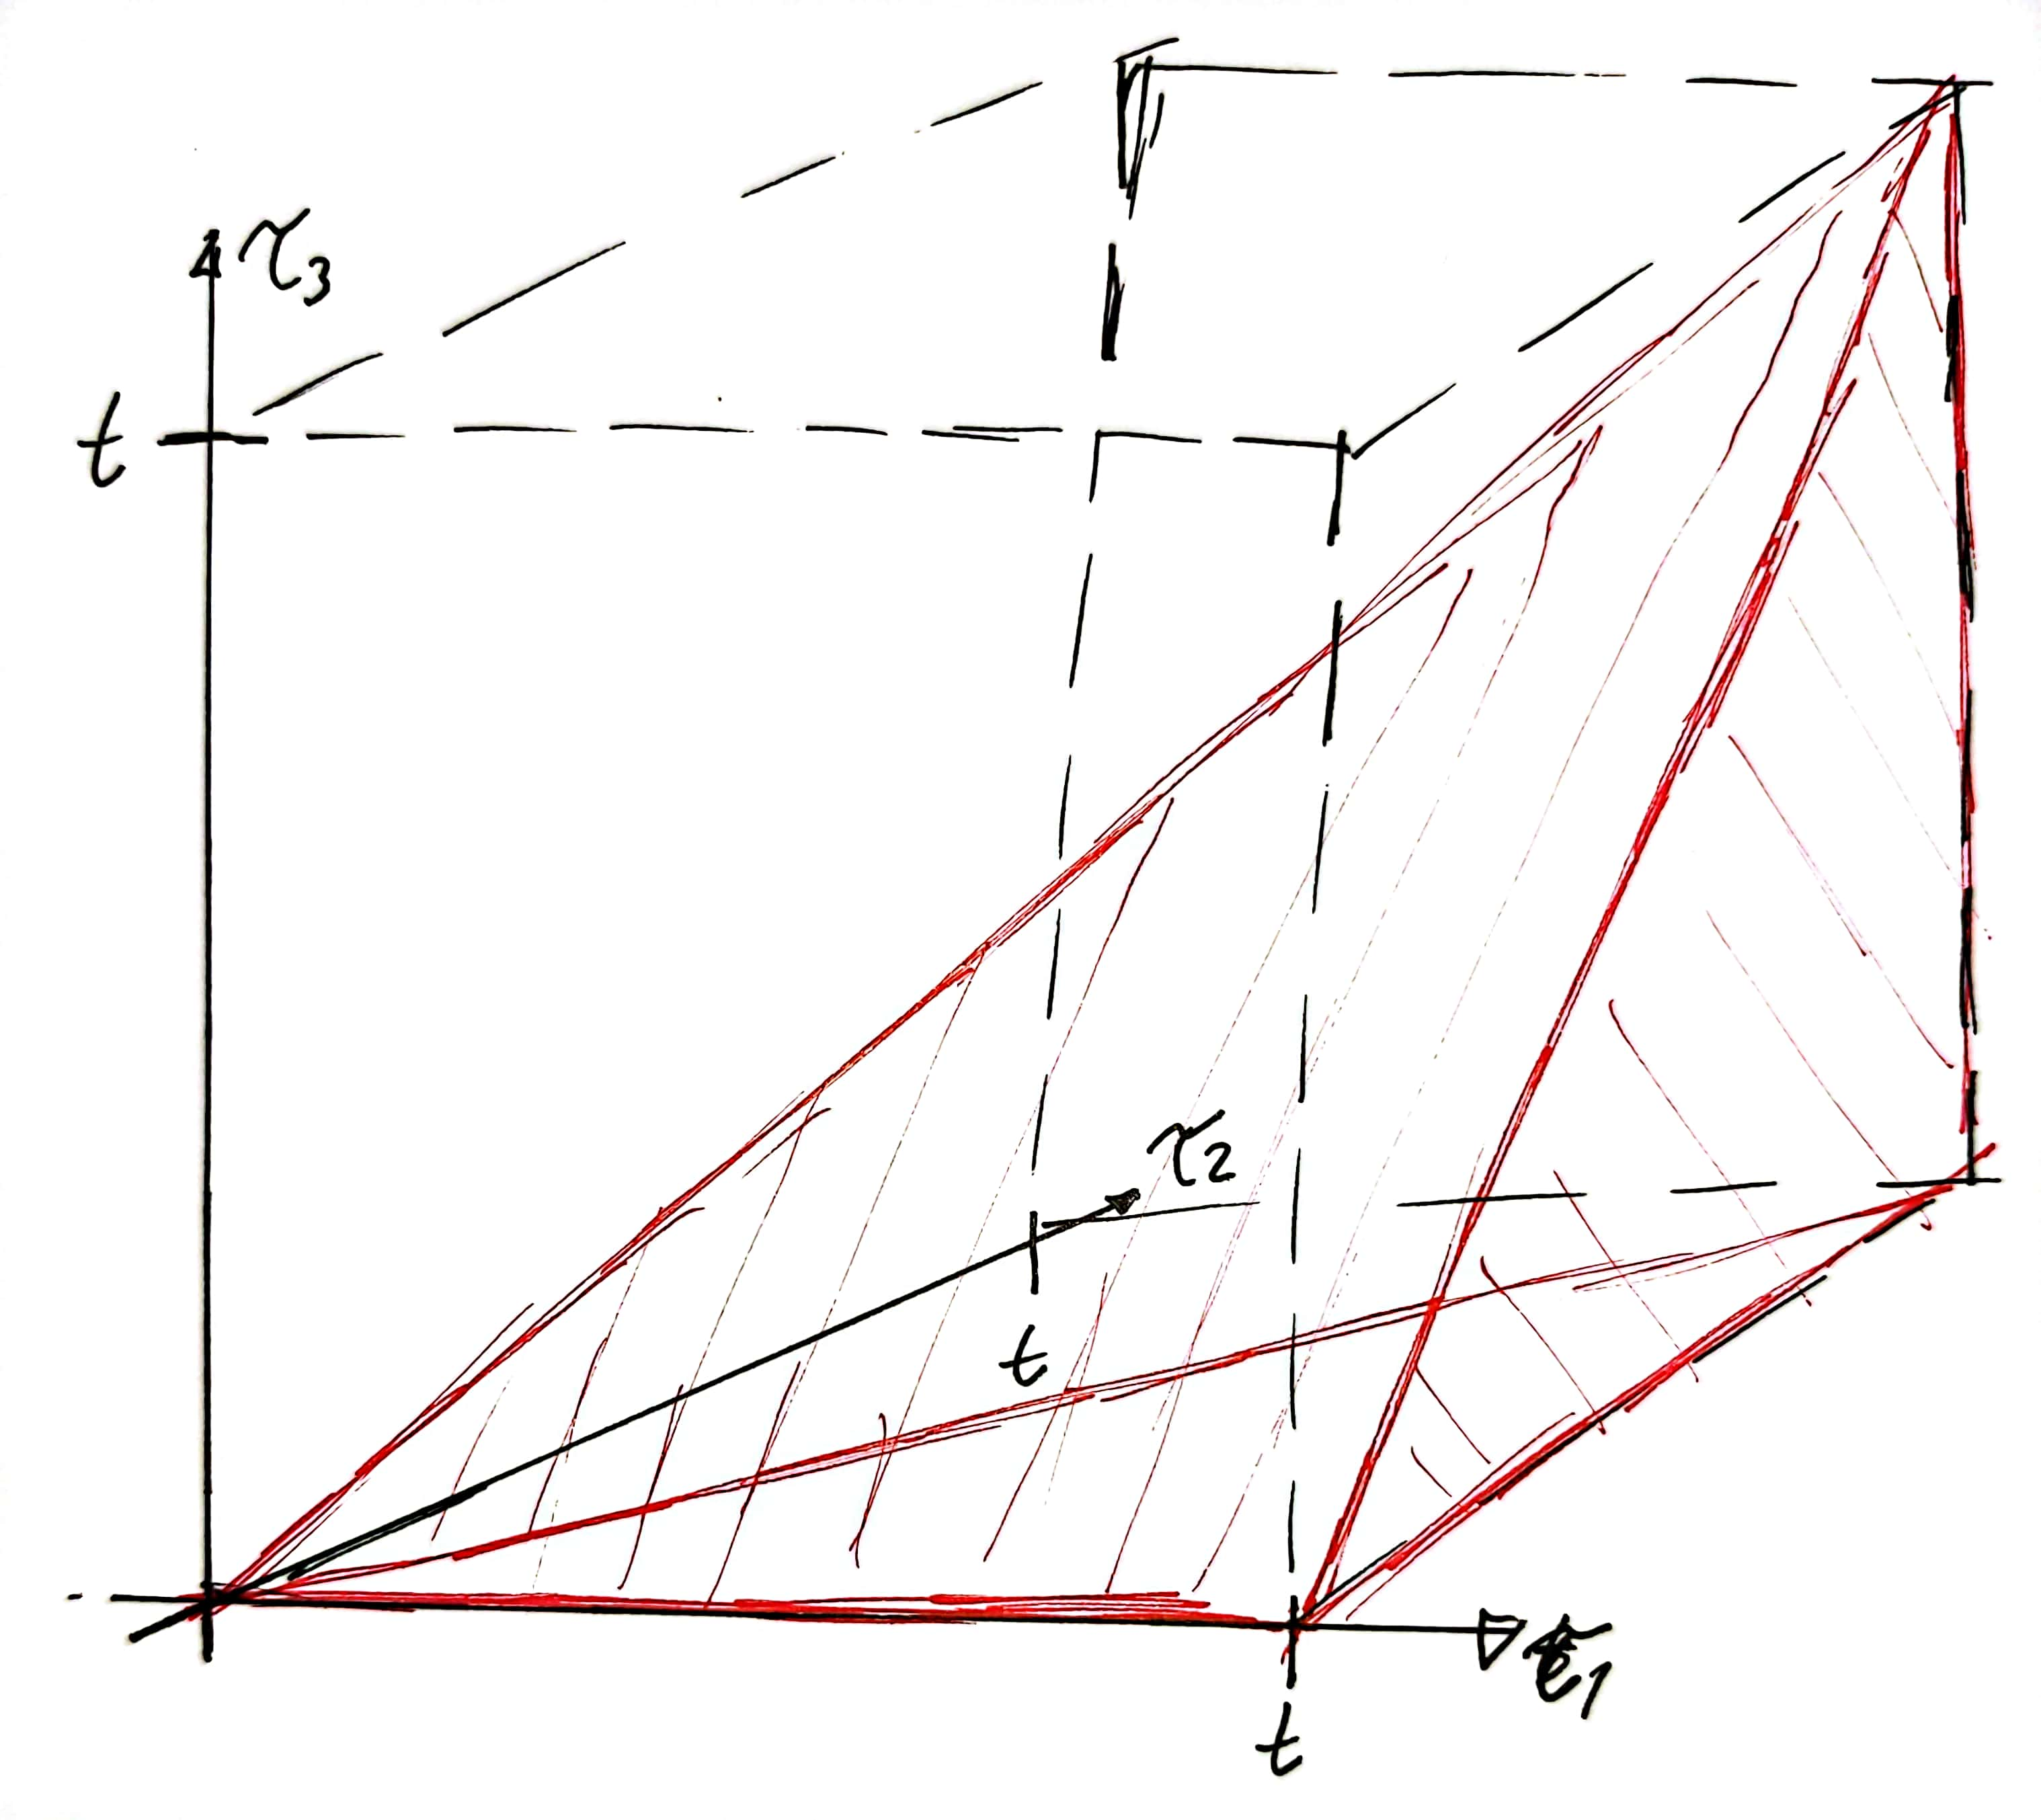
\includegraphics[width=.5\textwidth]{fig/time-ordering.jpg}
    \caption{We change the domain of integration from the cube to the smaller slice, illustrated in red.}
    \label{fig: time ordering}
\end{figure}

Adapting this formula to $W_n(x,t)$, we get the time-ordered integration
%
\begin{align}
    W_n(x, t) = 
    \int_0^t \dd \tau_1 \int_0^{\tau_1} \dd \tau_2 \cdots \int_0^{\tau_{N-1}} \dd \tau_N \, 
    \E{U(x(\tau_1)) U(x(\tau_2)) \cdots U(x(\tau_N)) }_{(x,t)}
\end{align}
%
Take then $n = 2$:
%
\begin{align}
    W_2(x, t) 
    &= \int_0^t \dd \tau_1 \int_0^{\tau_1} \dd \tau_2 \,
    \E{U(x(\tau_1)) U(x(\tau_2))}_{(x,t)} \\
    &
    = 
    \int_0^t \dd \tau_1 \int_0^{\tau_1} \dd \tau_2 
    \int \dd x_2 \int \dd x_1 \, 
    \Pe(x, t|x_1, \tau_1) U(x_1)   \Pe(x_1, \tau_1 | x_2, \tau_2) U(x_2) \Pe(x_2, \tau_2) \\
    & =
    \int_0^t \dd \tau_1 
    \int \dd x_1\,
    \Pe(x, t|x_1, \tau_1) U(x_1)   
     W_1(x_1, \tau_1) ,
\end{align}
%
where we used \autoref{eq: W_1}.
You may convince yourself that this recursive form holds in general---$W_n$ will always just add one more integral to $W_N$, so
%
\begin{align}
    W_n(x, t) = 
    \int_0^t \dd \tau_1 
    \int \dd x_1\,
    \Pe(x, t|x_1, \tau_1) U(x_1)   
    W_{n-1}(x_1, \tau_1) .
\end{align}
%
Next, we substitute the last relation into the expansion of $W(x, t)$, 
%
\begin{align}\label{eq:Wexp}
    W(x,t) = W_0(x, t) 
    - \sum_{n = 0}^\infty (-1)^n
    \int_0^t \dd \tau_1  \int \dd x_1 \,\Pe(x, t|x_1, \tau_1) U(x_1)   
    W_{n}(x_1, \tau_1).
\end{align}
%
This recursive integral expression for $W(x,t)$ is exact but impractical. In this spirit, we will use Eq. \eqref{eq:Wexp} to find a differential equation for $W(x,t)$.
We will use the fact that for the Brownian motion
%
\begin{align}
    \pdv{  }{ t } W_0(x, t) = D \pdv[2]{  }{ x } W_0(x, t), 
\end{align}
%
as $W_0 = \Pe$.
If we now take the time derivative of Eq. \eqref{eq:Wexp}, we get
%
\begin{align}
    &\pdv{  }{ t } W(x, t) 
    = D \pdv[2]{  }{ x } W_0(x, t)\\\nonumber
    & - \sum_{n = 0}^\infty (-1)^n
    \int \dd x_1\,
    \left\{
        \Pe(x, t|x_1, t) U(x_1)   
        W_{n}(x_1, t)
        +
        \int_0^t \dd \tau_1 
        \int \dd x_1\,
        \left[D \pdv[2]{  }{ x } \Pe(x, t|x_1, \tau_1) \right]
        U(x_1) 
        W_{n}(x_1, \tau_1)
    \right\}.
\end{align}
%
We have used that the conditional probability also obeys the Fokker-Planck equation in the last term in the curly brackets.
We then use $\Pe(x, t|x_1, t) = \delta(x - x_1)$, and the fact that we can pull out the spatial derivative, to obtain
%
\begin{align}
    \pdv{  }{ t } W(x, t) 
    &= 
    D \pdv[2]{  }{ x } 
    \left\{
    W_0(x, t)
    - \sum_{n = 0}^\infty (-1)^n
    \int_0^t \dd \tau_1 
    \int \dd x_1\,
     \Pe(x, t|x_1, \tau_1) U(x_1)
    W_{n}(x_1, \tau_1)
    \right\}\\
    & \quad
    - 
 U(x)   
    \sum_{n = 0}^\infty (-1)^n W_{n}(x, t) \\
    & = D \pdv[2]{  }{ x } W(x, t) - U(x) W(x, t).
\end{align}
%
Accordingly, we can express the solution of the above differential equation as the expectation value over the Wiener measure of a suitable exponential Brownian functional.
Moreover, note that for $t \rightarrow i t'$, we obtain the Schrödinger equation, again underlining the stochastic-quantum analogy.

This correspondence between a path integral and a partial differential equation,
%
\begin{align}
    \pdv{W(x, t)}{t} &= D \pdv[2]{ W(x, t) }{ x } - U(x) W(x, t)&
    &\iff&
    W(x, t) = \int\limits_{x(0) = 0}^{x(t) = x} \D x(t) \, \exp \left\{ - \int_0^t U(x(t)) \right\},
\end{align}
%
is called the Feynman-Kac formula.


\section{Application: First passage time}

As an application, we calculate the \emph{first passage time} of a Brownian particle $x(t)$.
This is the time $T$ such that $x = a > 0$, for some value $a$, \emph{for the first time}.
So, for a given realization $x$, there is some time $T$ such that $x(T) = a$ for the first time.
This varies by realization, and it thus has a cumulative distribution $\Pe_{\text{fp}}(T)$, which identifies the probability that the first passage time is smaller that a given value $T$.
This is related to the probability distribution of $x$ by
%
\begin{align}
    \Pe_\text{fp}(T > t) = \int_t^\infty \dd \tau \, p_\text{fp}(\tau) = 
    \Pe(x(\tau) < a,\, \forall \tau \in[0, t])
    \equiv \Pe( x < a, t),
\end{align}
which states that the probability for $T>t$ is equal to the fact that the particle position never crosses $a$ in the time interval $(0,t)$; $p_\text{fp}$ denotes the probability density of the first passage time.
%
Thus, by taking the derivative with respect to $t$ on both sides we get
%
\begin{align} \label{eq: first passage time}
    p_\text{fp}(t) =
    - \odv{  }{ t } \Pe_\text{fp}(T > t) =
    - \odv{  }{ t } \Pe(x < a, t).
\end{align}
%
We have reduced the problem of studying the statistics of the first passage time to that of a constrained Brownian motion.
Indeed, we may obtain $\Pe(x < a, t)$ by defining a Brownian integral.
Let us define the following Brownian functional
%
\begin{align}
    Q[x] &= \exp \left\{ - \int_0^t \dd \tau \, U(x(t)) \right\},
    &
    U(x) & = 
    \begin{cases}
        0 & x < a \\
        \infty & x \geq b .
    \end{cases}
\end{align}
%
Thus,
%
\begin{align}
    Q[x] & = 
    \begin{cases}
        1 & x(\tau) < a, \, \forall \tau < t \\
        0 & \text{else}.
    \end{cases}
\end{align}
%
This is because, if any of the points of the integral is infinite, the whole integral becomes infinite.
$Q[x]$ is thus an indicator functional for paths $x(t)$ that do \emph{not} pass $a$, and so
%
\begin{align}
    \Pe(x < a, t | x(t) = x) 
    = 
    \E{Q[x(t)]}_{(x, t)}.
\end{align}
%
This is the probability of not crossing $a$, condition on the endpoints.
The total probability is
%
\begin{align}\label{eq: first passage x}
    \Pe(x < a, t)
    = 
    \int \dd x'
    \E{Q[x(t)]}_{(x', t)}.
\end{align}
%
We can then find  $W(x, t) = \E{Q[x(t)]}_{(x, t)}$ using the Feynman-Kac formula, which says that $W$ is given by
%
\begin{align} \label{eq: feynman kac for first passage time}
    W(x, t) &= \int\limits_{x(0) = x}^{x(t) = x} \D x(t) \, \exp \left\{ - \int_0^t U(x(t)) \right\}, &
    U(x) & = 
    \begin{cases}
        0 & x < a \\
        \infty & x \geq b .
    \end{cases}.
\end{align}
%

\begin{framed}
    \textit{Exercise:}
    Calculate the Brownian integral $W(x, t)$ of \autoref{eq: feynman kac for first passage time} by solving the PDE.
    With this result, use \autoref{eq: first passage time} and \autoref{eq: first passage x} to find the probability density of the first-passage time, and its first moment.
\end{framed}

